\documentclass[dcc]{fcfmcourse}
\usepackage{teoria}
\usepackage[utf8x]{inputenc}
\usepackage{amsmath}
\usepackage{amsfonts,setspace}
\usepackage{listings}
\usepackage{color}
\usepackage{cancel}
\usepackage{epstopdf}
\usepackage{qtree}
\usepackage{fancyhdr}
\usepackage{tikz}
\usepackage{hyperref}
\usetikzlibrary{automata,positioning}
\pagestyle{fancy}
\cfoot{``Program testing can be used to show the presence of bugs, but never to show their absence!" \\Edsger Dijkstra}
\definecolor{pblue}{rgb}{0.13,0.13,1}
\definecolor{pgreen}{rgb}{0,0.5,0}
\definecolor{porange}{rgb}{0.9,0.5,0}
\definecolor{pgrey}{rgb}{0.46,0.45,0.48}

\lstset{language=Java,
  showspaces=false,
  showtabs=false,
  breaklines=true,
  showstringspaces=false,
  breakatwhitespace=true,
  commentstyle=\color{porange},
  keywordstyle=\color{pblue},
  stringstyle=\color{pgreen},
  basicstyle=\ttfamily,
  moredelim=[il][\textcolor{pgrey}]{$ $},
  moredelim=[is][\textcolor{pgrey}]{\%\%}{\%\%}
}

\newenvironment{codebox} {\small \ttfamily \obeylines \begingroup \setstretch{-2.4}} {\endgroup}

\title{Auxiliar Extra}
\course[CC3102]{Teoría de la Computación}
\professor{Gonzalo Navarro}
\assistant{Manuel Cáceres}
\assistant{Ian Letter}

% Si pasas el comando usedate a la clase, la fecha aparecerá bajo la lista de auxiliares.
% Puedes usar el formato de fecha por defecto de latex (y traducirla usando babel)
% o puedes escribir lo que quieras con el comando \date.
% \date{1 de Septiembre, 2015}

\begin{document}
\maketitle
\begin{center}
6 de Octubre del 2016
\end{center}
\vspace{-1ex}

\section*{Conversión GLC $\Leftrightarrow$ AP}
\begin{problems}
\problem Utilice la conversión GLC $\rightarrow$ AP para construir el autómata que reconoce la siguiente gramática:
\begin{center}
$S \rightarrow A\, | B\, | AB\, | BA$\\
$A \rightarrow a\, | aAa\, | aAb\, | bAb\,| bAa$\\
$B \rightarrow b\, | aBa\, | aBb\, | bBb\,| bBa$
\end{center}

\problem Utilice la conversión $AP \rightarrow GLC$, para construir la gramática correspondiente al siguiente autómata:\\
\begin{center}
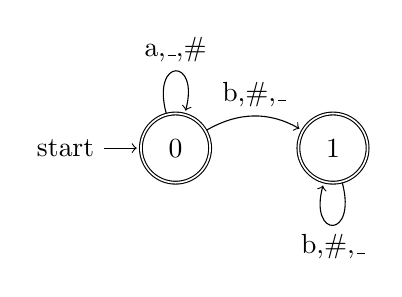
\begin{tikzpicture}[shorten >=1pt,node distance=2cm,on grid,auto] 
   \node[state,initial, accepting] (q_0)	{$0$}; 
   \node[state,accepting] (q_1) [right of=q_0]  {$1$}; 
    \path[->] 
    (q_0) edge [loop above] node  {a,\_,\#} (q_0)
    (q_0) edge [bend left] node  {b,\#,\_} (q_1)
    (q_1) edge [loop below] node  {b,\#,\_} (q_1);
\end{tikzpicture}
\end{center}
\end{problems}
\section*{Lema de Bombeo}
Si $\mathcal{L}$ es libre del contexto, entonces:
\begin{align*}
\exists N > 0, \forall w \in \mathcal{L}, &|w| > N \Rightarrow\\
&\exists x,u,y,v,z \in \Sigma^* (w=xuyvz \land uv \not = \epsilon \land |uyv|\le N \land \forall n \ge 0, xu^nyv^nz \in \mathcal{L})
\end{align*}

\begin{problems}
\problem Demuestre que los siguientes lenguajes no son libres del contexto:
\begin{enumerate}[a)]
    \item $\{a^p \colon p \text{ es primo}\}$
    \item $\{a^{n^2} \colon n \ge 0\}$
\end{enumerate}
\end{problems}
\newpage
\begin{center}
{\huge \underline{Soluciones}}
\end{center}
\section*{Conversión GLC $\Leftrightarrow$ AP}
\begin{problems}
\problem Este es el autómata resultante de la conversión:\\

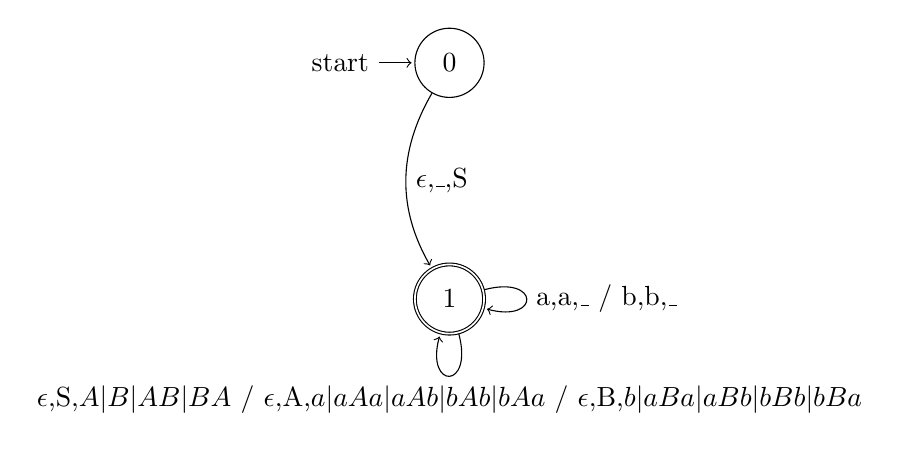
\begin{tikzpicture}[shorten >=1pt,node distance=3cm,on grid,auto] 
   \node[state,initial] (0)   {$0$}; 
   \node[state,accepting] (1) [below of=0]  {$1$}; 
    \path[->] 
    (0) edge [bend right] node  {$\epsilon$,\_,S} (1)
    (1) edge [loop right] node  {a,a,\_\ /\ b,b,\_} (1)
    (1) edge [loop below] node  {$\epsilon$,S,$A|B|AB|BA$\ /\  $\epsilon$,A,$a|aAa|aAb|bAb|bAa$\ /\ $\epsilon$,B,$b|aBa|aBb|bBb|bBa$} (1);
\end{tikzpicture}
\problem \textbf{Ejemplo 3.16} del apunte \url{https://www.dcc.uchile.cl/~gnavarro/apunte.pdf}
\end{problems}
\section*{Lema de Bombeo}
\begin{problems}
\problem 
\begin{enumerate}[a)]
\item Sea $N$ del lema de bombeo y escojamos un primo $p$ mayor a $N$ (existe pues hay infinitos primos).\\
Escogemos $a^p$ nuestra palabra y consideremos una división cualquiera de esta $a^p=xuyvz$. Digamos que $u = a^q$ y $v= a^t$ y además $r = |xyz| = p-q-t$.\\

En este caso bombeamos hasta $r$ quedando $|xu^ryv^rz| = r + rq + rt = r(1+q+t)$, el cual es compuesto siempre y cuando ambos factores sean mayores a $1$.
\begin{itemize}
\item Por un lado $q+t > 0$, por condición del lema de bombeo sobre $uv\ (\not = \epsilon)$ y por lo tanto $(1+q+t) > 1$
\item Por otro lado :
\begin{itemize}
\item Si $r=0$, se tiene que $xuyvz = uv$ y basta bombear a 2 de manera que $|u^2v^2| = 2p$ no es primo.
\item Si $r=1$, puedo bombear a $p+1$, esto es $|xu^{p+1}yv^{p+1}z| = 1+q(p+1)+t(p+1) = 1 + (q+t)(p+1) = 1 + (p-1)(p+1) = p^2$, que no es primo.
\end{itemize}
\end{itemize}
\newpage
\item Sea $N$ del lema de bombeo.\\
Escogemos $a^{N^2}$ nuestra palabra y consideremos una división cualquiera de esta \\$a^{N^2}=xuyvz$.\\
Las condiciones del lema de bombeo nos dicen que esta división cumplen con que $|uv|>0$ y $|uyv|\le N$, y por lo tanto $0<|uv|\le N$.\\
Si bombeamos a $2$ tenemos que $|xu^2yv^2z| = N^2 + k < N^2 + 2N + 1 = (N+1)^2$ que es el siguiente largo de palabra que está en lenguaje, por lo que $xu^2yv^2z$ no está en el lenguaje.
\end{enumerate}
\end{problems}

\end{document}
